\section{進階圖論}
    \subsection{DFS Tree}
    DFS Tree 是一個用來分析圖的一種方式,我們會對一張圖做DFS,
    然後對所有邊分類。

    \begin{figure}[!htbp]
        \centering
        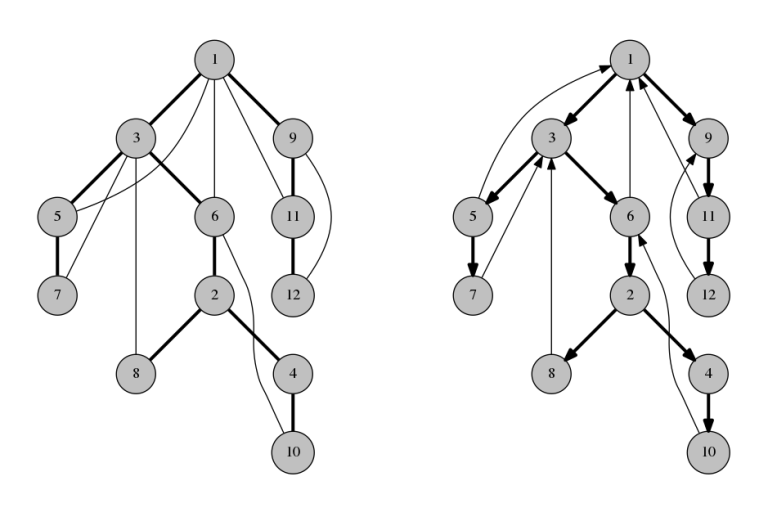
\includegraphics[width=0.8\textwidth]{../Images/AT1.png}
    \end{figure}

    如果是無向圖,則我們可以將邊分為兩類。

    \begin{itemize}
        \item Tree Edge :到達的點在DFS過程中是第一次被拜訪。
        \item Back Edge:到達的點在DFS過程中\textbf{不}是第一次被拜訪。
    \end{itemize}

    而如果是有向圖,則我們可以將邊分為四類。

    \begin{itemize}
        \item Tree Edge :到達的點在DFS過程中是第一次被拜訪。
        \item Back Edge :到達的點在他出發點的上面(深度較小,且共同祖先就是其中一個點)
        \item Forward Edge :到達的點在他出發點的下面(深度較大,且共同祖先就是其中一個點)
        \item Cross Edge :不同家族間的邊。(共同祖先\textbf{不}是其中一個點)
    \end{itemize}

    \begin{figure}[!htbp]
        \centering
        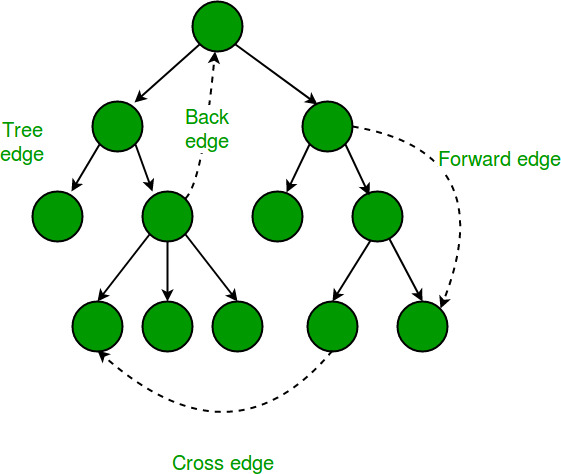
\includegraphics[width=0.8\textwidth]{../Images/AT2.png}
    \end{figure}

    有一些性質可以從DFS Tree得到。例如環,如果一個邊是Back Edge,
    那他一定有環經過這個邊,如果他是Cross Edge,則有可能有環在上面,
    且必定經過至少兩個Cross Edge或Back Edge。

    \subsection{邊雙連通分量}
    介紹邊雙連通分量前,我們應該要先介紹邊雙聯通的定義。如果我們說點$a$到點$b$為
    邊雙連通,那麼就算我們刪掉這張圖的任何一條邊也不會影響$a$與$b$的聯通性。

    邊雙連通滿足遞移律,也就是如果$a$到$k$邊雙連通,且$k$到$b$也邊雙連通,
    那麼$a$到$b$就會邊雙連通。

    在這個情況下我們會有一個新的名詞,橋(Bridge / Cut Edge),就是
    如果沒有他整張圖就沒有連通的邊。

    倘若我們想要找到所有的橋,我們就會需要一個新的演算法-Tarjan算法。
    
    \begin{figure}[!htbp]
        \centering
        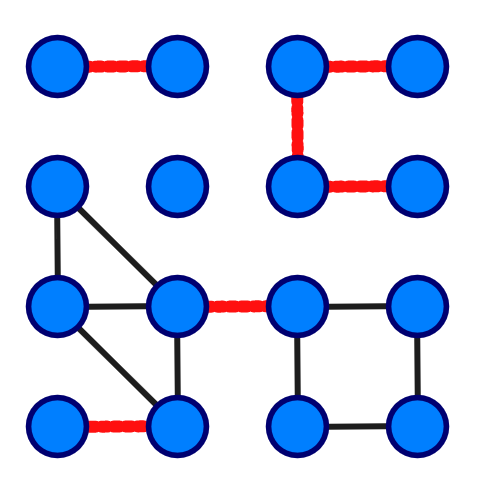
\includegraphics[width=0.5\textwidth]{../Images/AT3.png}
    \end{figure}

    小插曲:有許多他發明的演算法都以他的名字命名,所以有時候會讓人混淆。

    具體來說,我們可以運用DFS Tree,首先,Back Edge一定不是橋,因為
    所有的Tree Edge一定會讓剩餘圖連通(對於每一個連通分量而言)。

    那怎麼判斷Tree Edge是不是橋,我們需要有一個新的函數:$low(v)$。

    $$low(v) := 在不透過v的父邊的情況下,能夠到達深度最淺的祖先的深度$$

    另一個原來就有的函數是$dep(v)$,就是他在樹上的深度,也是到根節點的距離。

    如果$low(v)=dep(v)$,則他的父邊就是橋。而$low(v)$可以用DP求得。

\begin{lstlisting}[caption=邊雙連通]
const int N=100010;
vector<int> g[N];
bool vis[N],bridge[N];
int low[N],dep[N];
 
void dfs(int x){
    vis[x]=true;
    low[x]=dep[x];
    for(auto i:g[x]){
        if(vis[i]){
            low[x]=min(low[x],dep[i]);
        }else{
            dep[i]=dep[x]+1;
            dfs(i);
            low[x]=min(low[x],low[i]);
        }
    }
    if(low[x]==dep[x]) bridge[x]=true;
}
\end{lstlisting}

    \subsection{其他東西}
    油漆未乾,請轉駕至 \url{https://hackmd.io/@Ccucumber12/HylySg2xF#}

    \begin{figure}[!htbp]
        \centering
        
\includegraphics[width=0.2\textwidth]{../Images/AT4.png}
    \end{figure}